%%%%%%%%%%%%%%%%%%%%%%%%%%%%%%%%%%%%%%%%%%%%%%%%%%%%%%%%%%%%%%%%%%% 
%                                                                 %
%                            CHAPTER                              %
%                                                                 %
%%%%%%%%%%%%%%%%%%%%%%%%%%%%%%%%%%%%%%%%%%%%%%%%%%%%%%%%%%%%%%%%%%% 

\chapter{Platforms for accelerating Smith-Waterman}
\label{ch:Platforms}

As we saw in the analysis of the Smith-Waterman algorithm in \ref{expl:SWanalyse}, we can see that the value of each cell in the matrix is only dependent on the left-upmost 3 cells. Therefore, It leads us to believe that this algorithm can be accelerated on other hardware solutions which are better equipped for parrallellism than a normal CPU.

\section{Overview of possible hardware}

When designing a processing unit based on semiconductor technologies, it is always a tradeoff between efficiency and flexibility. For example, the CPU in a PC should be flexible so that it can run any set of instructions without a lot of intervention between changes. On the other hand, if a certain algorithm or instructionset should be executed as fast as possible, the FPGA's and ASICs are the best choice. At the extreme, an ASIC or \emph{Application Specific Integrated Circuit} can be chosen, but this means a complete chip should be designed from the ground up just for this specific application. This means that an ASIC is extremely expensive to design and build, especially for small production quantities. In figure \ref{fig:effVSflex} an overview of the different options can be found.

\begin{figure}[H]
	%src=https://docs.microsoft.com/en-us/azure/machine-learning/service/media/concept-accelerate-with-fpgas/azure-machine-learning-fpga-comparison.png
	\centering
	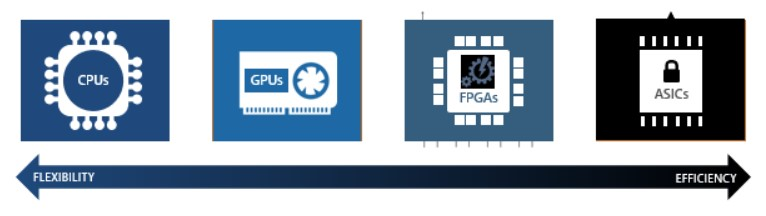
\includegraphics[width=0.75\textwidth]{elBackground/effVSflex.jpg}
	\caption{An overview of the different semiconductor technologies}
	\label{fig:effVSflex}
\end{figure}

\subsection{CPU}

The power of the CPU is it's flexibility: it can very easily be programmed with new instructions in very few time. However, if the CPU would only run one specific algorithm for its whole lifetime, it would be terribly inefficient. Also, CPU's work sequentially, which is less suitable for algorithms which demand a large amount of computations which could be done in parallel.

\begin{figure}[H]
	%src=http://www.lighterra.com/papers/modernmicroprocessors/sequential2.png
	\centering
	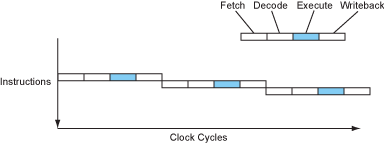
\includegraphics[width=0.75\textwidth]{elBackground/CPU.png}
	\caption{A cpu processes instructions sequentially. It could be accelerated using pipelining, but the maximum stays 1 instruction per clock cycle}
	\label{fig:cpu}
\end{figure}

Since the original implementations on CPU, it became clear that a CPU was not the most suitable platform for the S-W algorithm, since it consists of a lot of operations which can be done in parallel. However, since the rise SIMD, CPU's have made a comeback. \emph{SIMD} stands for \emph{Single Instruction Multiple Data} and makes it possible to manipulate more than 1 attribute of data with one single instruction, although be it the same instruction on all the data. CLC bio, a Danish company specialised in bioinformatics, has been able to achieve impressive speedups with a software implementation using SIMD, closing in on 200x.
%src:https://web.archive.org/web/20070811101052/http://www.clccell.com/download.html

Nowadays, MIT has published \emph{diagonalsw}, which an implementation of S-W using the SIMD instruction set, and is licensed under the open-source MIT license.

\subsection{GPU}

a GPU, or \emph{Graphical Processing Unit} is a semiconductor technology that is specialized in video encoding and decoding, which means it is especially built for matrix manipulations. Since the Smith-Waterman algorithm is basically a big matrix manipulation, it lead researchers to believe that it could be accelerated on a GPU. In 1997, an implementation of S-W on a GPU was published %src:  https://archive.org/details/computationalsci0000iccs_y9o8/page/230
which achieved a speedup of 2x over all previous software implementations.

At the time of writing, 11 different implementations for Smith Waterman have been reported, 3 of which reporting a speedup over 30 times.

\subsection{FPGA}

an FPGA, or \emph{Field Programmable Gate Array}, is an integrated circuit consisting of programmable logic components. These logic components can be programmed as any logic function, such as AND, XOR, etc. In most FPGA other elements are also found, such as memory blocks, DSP blocks, etc.

In the most basic FPGA's, the following items are definitely present:
\begin{enumerate}
	\item CLB's, or \emph{Complex Logic Blocks}, consisting of a \emph{LookUp Table} (LUT) and a flipflop. A LUT can be programmable so that it contains any type of logic function.
	\item Programmable Interconnects have to connect the CLB's into a bigger circuit, which is also called \emph{routing}. This routing has the most influence on delays, and are also responsible for most errors.
	\item I/O blocks, which connect the internal logic inside with the outside pins of the FPGA. Most can be configured as input, output or bidirectional.
\end{enumerate}

\begin{figure}[H]
	%src=https://evergreen.loyola.edu/dhhoe/www/FPGA_diagram.png
	\centering
	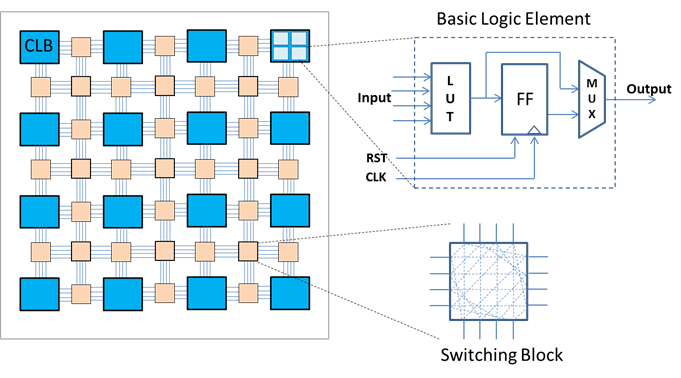
\includegraphics[width=0.75\textwidth]{elBackground/FPGA.png}
	\caption{The basic layout of an FPGA}
	\label{fig:fpga}
\end{figure}

For an implementation or design of a circuit which should be loaded in an FPGA, a \emph{Hardware Description Language} (HDL) is often the only practical choise to implement such a system, since drawing the circuits with a CAD program or by hand would take a very long time.

In a paper form 2007, an implementation of S-W with an FPGA (virtex-4) achieved a speedup up to 100x in comparison with a 2.2GHz Opteron processor. %src https://ft.ornl.gov/~olaf/pubs/RSSIOlafDave.pdf
A few companies also have made some implementations of FPGA in the past, e.g. Cray Inc., TimeLogics, ...
%cray: https://www.cray.com/
%timelogics: http://www.timelogic.com/

A master's thesis from 2011 by Vermij E. has a detailed analysis of an FPGA based Smith-Waterman implementation. In other papers, it was found that the performance per Watt level for an FPGA implementation is better than a GPU or CPU by a factor of 12-21 times.

\section{Hardware selection}

\subsection{Recent advances in High Level Synthesis}

\subsection{Platform communication}
niet belangrijk
via SD
ev. Ethernet: FTP

reading from sd card so not a lot of information exchange needed
if necessary => FTP if needed

